\chapter[\textit{uv}]{\textit{uv} \\ Pour une gestion avancée \\ des environnements \\ de développement}

\insertcitation{Il y a un moyen de faire mieux, trouvez-le.}{Thomas Edison}
\bigskip

\textbf{uv} est un gestionnaire de dépendances ainsi qu'un outil de \textit{packaging} conçu pour offrir une performance optimale, tout en se révélant être d'une grande simplicité au niveau de son utilisation. \textbf{uv} se distingue par sa capacité à résoudre rapidement (écrit en \textbf{Rust}\footnote{\url{https://www.rust-lang.org/fr}} une attention fut portée sur la rapidité d'exécution) les dépendances et à créer des environnements virtuels de manière transparente.

Dans ce chapitre, nous allons explorer les grandes lignes de l'outil \textbf{uv} et découvrir comment il peut transformer notre approche du développement Python. Nous commencerons par une introduction à ses fonctionnalités de base, puis nous plongerons dans des aspects plus avancés, tels que la gestion des environnements virtuels, la résolution des dépendances, et le \textit{packaging} de projets, optimisant ainsi notre flux de travail.

Cet outil saura certainement devenir un allié incontournable, voire indispensable, pour notre boîte à outils de développement Python.

\section{Présentation d'\textit{uv}}
L'idée principale d'\textbf{uv} est d'accélérer le flux en accélérant les actions de gestion de projet. Par exemple, pour l'installation de paquets, \textbf{uv} est dix à cent fois plus rapide que \textbf{pip}.

\begin{figure}[h!]
    \centering
    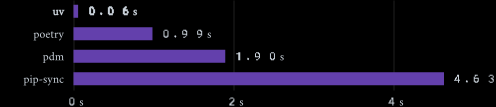
\includegraphics[width=0.7\textwidth]{IMG/uv_graph.png} % Remplacez par le chemin de votre image
    \caption{Graphique illustrant la rapidité, tiré de la documentation officielle}
\end{figure}

En outre, \textbf{uv} intègre dans un seul outil la plupart des fonctionnalités fournies par des outils tels que \textbf{pip}, \textbf{pip-tools}, \textbf{pipx}, \textbf{poetry}, \textbf{pyenv}, \textbf{twine}\footnote{\url{https://twine.readthedocs.io/en/stable/index.html}}, \textbf{virtualenv}, et bien d'autres encore. \textbf{uv} est donc une solution tout-en-un.

Caractéristiques d'\textbf{uv} :
\begin{itemize}
    \item Installation rapide des dépendances
    \item Gestion des environnements virtuels
    \item Gestion des versions de Python
    \item Initialisation du projet : Permet d'échafauder un projet Python complet, y compris le répertoire racine, le dépôt \textbf{Git}, l'environnement virtuel, \texttt{pyproject.toml}, \texttt{README}, etc.
    \item Gestion des dépendances pour une reproductibilité de l'environnement
    \item Gestion de la construction et de la publication des paquets
    \item Prise en charge des outils de développement : Installe et permet d'exécuter des outils de développement, tels que \textbf{pytest}\footnote{\url{https://docs.pytest.org/en/stable/}}, \textbf{Black}\footnote{\url{https://pypi.org/project/black/}} et \textbf{Ruff}\footnote{\url{https://docs.astral.sh/ruff/}}.
\end{itemize}
\medskip

Site officiel : \url{https://docs.astral.sh/uv/}

Serveur \textbf{Discord} : \url{https://discord.gg/JSsj35HH}

\section{Installation}
La façon la plus rapide (bien plus rapide) d'installer \textbf{uv} est d'utiliser l'installateur autonome fournit par le projet \textbf{uv}. Une autre option est d'installer \textbf{uv} à partir de \textbf{PyPI} en utilisant d'autres outils comme \textbf{pipx} ou \textbf{pip}\footnote{Pour d'autres modes d'installation voir la documentation officielle : \url{https://docs.astral.sh/uv/getting-started/installation/}}.

Pour installer la dernière version d'\textbf{uv} (sous forme de binaires) :
\begin{lstlisting}[style=bash]
|\userprompt| curl -LsSf https://astral.sh/uv/install.sh |\textbar| sh
downloading uv 0.7.8 x86_64-unknown-linux-gnu
no checksums to verify
installing to /home/user/.local/bin
  uv
  uvx
everything's installed!
\end{lstlisting}

Il est cependant possible d'obtenir une version spécifique d'\textbf{uv}\footnote{Voir la page \textbf{GitHub} des différentes versions : \url{https://github.com/astral-sh/uv/releases}} en incluant le numéro de version dans l'\textit{URL} :
\begin{lstlisting}[style=bash]
|\userprompt| curl -LsSf https://astral.sh/uv/0.7.7/install.sh |\textbar| sh
downloading uv 0.7.7 x86_64-unknown-linux-gnu
no checksums to verify
installing to /home/krystof/.local/bin
  uv
  uvx
everything's installed!
\end{lstlisting}

Vérifier l'installation :
\begin{lstlisting}[style=bash]
|\userprompt| uv --version 
uv 0.7.7
\end{lstlisting}

Activer l'auto-complétion dans \textbf{zsh}, à la fois pour \textbf{uv} et \textbf{uvx} :
\begin{lstlisting}[style=bash]
|\userprompt| echo 'eval "$(uv generate-shell-completion zsh)"' >> ~ /.zshrc
|\userprompt| echo 'eval "$(uvx generate-shell-completion zsh)"' >> ~/.zshrc
\end{lstlisting}

\subsection*{Mise à jour d'\textit{uv}}
Comme le projet \texttt{uv} est en développement actif, de nouvelles versions sont régulièrement publiées. Si \textbf{uv} a été installé à l'aide de l'installateur autonome il sera nécessaire d'exécuter la commande suivante :
\begin{lstlisting}[style=bash]
|\userprompt| uv self update
info: Checking for updates...
success: Upgraded uv from v0.7.7 to v0.7.8! https://github.com/astral-sh/uv/releases/tag/0.7.8
\end{lstlisting}

\subsection*{Désinstallation}
Nettoyer les données stockées :
\begin{lstlisting}[style=bash]
|\userprompt| uv cache clean
No cache found at: .cache/uv  # Normal au début
|\userprompt| rm -r "$(uv python dir)"
|\userprompt| rm -r "$(uv tool dir)"
\end{lstlisting}

Supprimer les binaires \textbf{uv} et \textbf{uvx} :
\begin{lstlisting}[style=bash]
|\userprompt| rm ~/.local/bin/uv ~/.local/bin/uvx
|\userprompt| uv --version
zsh: command not found: uv
\end{lstlisting}

\subsection*{Un aperçu rapide}
Maintenant qu'\textbf{uv} est installé prenons le temps de visualiser très rapidement ce que cet outil a à nous proposer :
\begin{lstlisting}[style=bash]
|\userprompt| uv
An extremely fast Python package manager.

Usage: uv [OPTIONS] <COMMAND>

Commands:
  run      Run a command or script
  init     Create a new pyproject
# Saisir la commande pour voir la suite de la sortie...
\end{lstlisting}

Pour accéder à l'aide d'une commande d'\textbf{uv} :
\begin{lstlisting}[style=bash]
|\userprompt| uv --help <commande>
\end{lstlisting}

Par exemple, la commande \texttt{cache} :
\begin{lstlisting}[style=bash]
|\userprompt| uv --help cache
\end{lstlisting}

Cela permet d'ouvrir un visualisateur dans lequel on retrouve les informations sollicitées (ce qui suit n'est qu'un extrait) :
\begin{lstlisting}[style=visual]
Manage uv's cache

Usage: uv cache [OPTIONS] <COMMAND>

Commands:
  clean  Clear the cache, removing all entries or those linked to specific packages
  prune  Prune all unreachable objects from the cache
  dir    Show the cache directory
|\textcolor{nord4}{[...]}|
\end{lstlisting}

\section{La gestion de projet}

Pour cette section et la suite du didacticiel, nous utiliserons un exemple d'application qui permet d'afficher un calendrier à l'aide d'une interface graphique créée via le \textit{framework} \textbf{Qt for Python}\footnote{\url{https://doc.qt.io/qtforpython-6/}, alias \textbf{PySide6} : \url{https://pypi.org/project/PySide6/}}. Le code de cette application se trouve sur un dépôt \textbf{GitHub}\footnote{\url{https://github.com/Krystof2so/PyCalendar} - Voir également l'annexe \textit{Code du projet \textbf{Calendar}} page \pageref{code_calendar}}. Il s'agit d'un petit projet personnel réalisé au cours de mon apprentissage du \textit{framework}, mais rien ne vous empêche de tester toutes les manipulations qui vont suivre à partir de tout autre projet. Le projet \textbf{Calendar} ne me sert qu'à illustrer mon propos.

Créer et travailler sur des projets Python avec \textbf{uv}, revient à travailler avec le fichier \texttt{pyproject.toml}, fichier qui, comme nous l'avons vu dans les chapitres précédents, définit les dépendances.

\subsection*{Création d'un projet}

Pour créer et initialiser un projet Python avec \textbf{uv}, naviguer jusqu'au répertoire dans lequel on souhaite stocker le projet (par exemple le répertoire personnel de l'utilisateur), puis exécuter la commande :
\begin{lstlisting}[style=bash]
|\userprompt| uv init mon_projet
Initialized project `mon_projet` at `/home/utilisateur/mon_projet`
\end{lstlisting}

ou bien :
\begin{lstlisting}[style=bash]
|\userprompt| mkdir mon_projet
|\userprompt| cd mon_projet
|\userprompt| uv init
Initialized project `mon_projet`
\end{lstlisting}

Cela crée dans le répertoire du projet (\texttt{mon\_projet}) la structure suivante :
\begin{lstlisting}[style=tree]
mon_projet/
|\textbar|
|\textbar|--.python-version
|\textbar|--README.md
|\textbar|--main.py
|\textbar|--pyproject.toml
\end{lstlisting}

Le fichier \texttt{.python-version} contient la version de Python par défaut pour le projet en cours. Ce fichier indique à \textbf{uv} la version de Python à utiliser lors de la création d'un environnement virtuel dédié au projet. Ensuite, il y a un fichier \texttt{README.md}.  Et l'on trouve un fichier \texttt{main.py} qui contient les lignes suivantes :
\begin{lstlisting}[style=python]
def main():
    print("Hello from mon-projet!")


if __name__ == "__main__":
    main()
\end{lstlisting}

Et au final un fichier \texttt{pyproject.toml} initié avec une configuration basique :
\begin{lstlisting}[style=file]
[project]
name = "mon-projet"
version = "0.1.0"
description = "Add your description here"
readme = "README.md"
requires-python = ">=3.13"
dependencies = []
\end{lstlisting}

Nous pouvons changer la description :
\begin{lstlisting}[style=file]
description = "Un simple projet"
\end{lstlisting}


\subsection*{Initier un projet existant}
Nous allons pour cela utiliser le projet \textbf{Calendar}\footnote{Cf. annexe \textit{Code du projet \textbf{Calendar}} page \pageref{code_calendar}}. Il suffit tout simplement de se rendre dans le répertoire du projet et de lancer la commande \texttt{init} :
\begin{lstlisting}[style=bash]
|\userprompt| uv init
Initialized project `calendar`
|\userprompt| tree  
.
|\textbar|-- IMG
|\textbar|   |\textbar|-- PyCalendar.png
|\textbar|-- main.py
|\textbar|-- pyproject.toml
|\textbar|-- README.md
|\textbar|-- src
|\textbar|-- pycalendar
        |\textbar|-- main.py

4 directories, 5 files
\end{lstlisting}

Cette commande va seulement générer le fichier \texttt{pyproject.toml}. Elle ne va ni écraser, ni modifier les fichiers existants, ni modifier la structure du projet. Cependant, cette commande ne fonctionnera pas si un fichier \texttt{pyproject.toml} est déjà présent. Si c'est le cas, copier le fichier avant de lancer la commande \texttt{uv init}, il pourra servir pour modifier le nouveau fichier généré avec toute configuration pertinente de l'ancien \texttt{pyproject.toml}.

\subsection*{Exécution du script d'entrée du projet}
\begin{lstlisting}[style=bash, escapeinside={||}]
|\userprompt| uv run main.py
Using CPython 3.13.3 interpreter at: /usr/bin/python3.13
Creating virtual environment at: .venv
Hello from calendar!
|\userprompt| tree -a
.
|\textbar|-- main.py
|\textbar|-- pyproject.toml
|\textbar|-- .python-version
|\textbar|-- README.md
|\textbar|-- uv.lock
|\textbar|-- .venv
    |\textbar|-- bin
    |\textbar|   |\textbar|-- activate
    |\textbar|   |\textbar|-- activate.bat
    |\textbar|   |\textbar|-- activate.csh
    |\textbar|   |\textbar|-- activate.fish
    |\textbar|   |\textbar|-- activate.nu
    |\textbar|   |\textbar|-- activate.ps1
    |\textbar|   |\textbar|-- activate_this.py
    |\textbar|   |\textbar|-- deactivate.bat
    |\textbar|   |\textbar|-- pydoc.bat
    |\textbar|   |\textbar|-- python -> /usr/bin/python3.13
    |\textbar|   |\textbar|-- python3 -> python
    |\textbar|   |\textbar|-- python3.13 -> python
    |\textbar|-- CACHEDIR.TAG
    |\textbar|-- .gitignore
    |\textbar|-- lib
    |\textbar|   |\textbar|-- python3.13
    |\textbar|       |\textbar|-- site-packages
    |\textbar|           |\textbar|-- __pycache__
    |\textbar|           |\textbar|   |\textbar|-- _virtualenv.cpython-313.pyc
    |\textbar|           |\textbar|-- _virtualenv.pth
    |\textbar|           |\textbar|-- _virtualenv.py
    |\textbar|-- lib64 -> lib
    |\textbar|-- pyvenv.cfg

8 directories, 23 files
\end{lstlisting}

La première fois que l'on exécutez une commande de projet, soit \texttt{uv run}, \texttt{uv sync} (création de l'environnement du projet) ou \texttt{uv lock}, la version de Python utilisée pour le projet est affichée. \textbf{uv} crée ensuite un environnement virtuel et un fichier \texttt{uv.lock} (cf. infra) à la racine du projet, ainsi qu'un fichier \texttt{.gitignore}, installé dans le répertoire de gestion de l'environnement virtuel (\texttt{.venv}) dont le contenu est vide. 

Si l'on ne souhaite pas qu'\textbf{uv} gère l'environnement du projet, désactiver le verrouillage et la synchronisation automatiques du projet dans \texttt{pyproject.toml} :
\begin{lstlisting}[style=file]
[tool.uv]
managed = false
\end{lstlisting}

Ce qui donnera à la première exécution :
\begin{lstlisting}[style=bash]
|\userprompt| uv run main.py
Hello from mon_projet!
|\userprompt| tree -a
.
|\textbar|-- main.py
|\textbar|-- pyproject.toml
|\textbar|-- .python-version
|\textbar|-- README.md

1 directory, 4 files
\end{lstlisting}

\section{La gestion des dépendances}
\subsection*{Ajout et installation des dépendances}
Revenons au projet \textbf{Calendar} :
\begin{lstlisting}[style=bash]
|\userprompt| cd calendar
|\userprompt| uv init
Initialized project `calendar`
|\userprompt| uv run src/pycalendar/main.py
Using CPython 3.13.3 interpreter at: /usr/bin/python3.13
Creating virtual environment at: .venv
Traceback (most recent call last):
  File "/home/utilisateur/calendar/src/pycalendar/main.py", line 4, in <module>
    from PySide6.QtCore import QSize, Qt
ModuleNotFoundError: No module named 'PySide6'
\end{lstlisting}

L'exception levée est sans appel : il nous manque un module nécessaire pour exécuter correctement notre application, le module \textbf{PySide6}. Remédions à cela:
\begin{lstlisting}[style=bash]
|\userprompt| uv add pyside6
Resolved 5 packages in 443ms
Prepared 4 packages in 10.63s
Installed 4 packages in 146ms
 + pyside6==6.9.0
 + pyside6-addons==6.9.0
 + pyside6-essentials==6.9.0
 + shiboken6==6.9.0
\end{lstlisting}

Ou bien en spécifiant une version précise du module :
\begin{lstlisting}[style=bash]
|\userprompt| uv add "pyside6==6.9.0"
Resolved 10 packages in 16ms
Installed 4 packages in 117ms
 + pyside6==6.9.0
 + pyside6-addons==6.9.0
 + pyside6-essentials==6.9.0
 + shiboken6==6.9.0
\end{lstlisting}

Ces commandes permettent d'ajouter la bibliothèque \textbf{PySide6} aux dépendances du projet et de l'installer dans l'environnement virtuel. Le fichier \texttt{pyproject.toml} est alors modifié en conséquence :
\begin{lstlisting}[style=file]
[project]
name = "calendar"
version = "0.1.0"
description = "Simple calendar"
readme = "README.md"
requires-python = ">=3.13"
dependencies = [
    "pyside6>=6.9.0",
]
\end{lstlisting}

Il est même possible d'ajouter une dépendance depuis un projet \textbf{GitHub} (par exemple , le module \textbf{requests}) :
\begin{lstlisting}[style=bash]
|\userprompt| uv add git+https://github.com/psf/requests
    Updated https://github.com/psf/requests (c65c780849563c891f35ffc98d3198b71011c012)
Resolved 15 packages in 364ms
      Built requests @ git+https://github.com/psf/requests@c65c780849563c891f35ffc98d3198b71011c 012
Prepared 5 packages in 891ms
Installed 5 packages in 7ms
 + certifi==2025.4.26
 + charset-normalizer==3.4.2
 + idna==3.10
 + requests==2.32.3 (from git+https://github.com/psf/requests@c65c780849563c891f35ffc98d3198b71011c012)
 + urllib3==2.4.0
\end{lstlisting}

Si le projet possédait déjà un fichier \texttt{requirements.txt} : 
\begin{lstlisting}[style=file]
PySide6==6.9.0
PySide6_Addons==6.9.0
PySide6_Essentials==6.9.0
shiboken6==6.9.0
\end{lstlisting}

Il suffisait alors d'en passer par lui :
\begin{lstlisting}[style=bash]
|\userprompt| uv add -r requirements.txt
Using CPython 3.13.3 interpreter at: /usr/bin/python3.13
Creating virtual environment at: .venv
Resolved 5 packages in 1ms
Installed 4 packages in 91ms
 + pyside6==6.9.0
 + pyside6-addons==6.9.0
 + pyside6-essentials==6.9.0
 + shiboken6==6.9.0
\end{lstlisting}

Et notre nouveau \texttt{pyproject.toml}:
\begin{lstlisting}[style=file]
[project]
name = "calendar"
version = "0.1.0"
description = "Add your description here"
readme = "README.md"
requires-python = ">=3.13"
dependencies = [
    "pyside6==6.9.0",
    "pyside6-addons==6.9.0",
    "pyside6-essentials==6.9.0",
    "shiboken6==6.9.0",
]
\end{lstlisting}

\textit{uv add} met également à jour le fichier \texttt{uv.lock} avec les informations de version pour les éléments suivants :
\begin{description}
    \item[Dépendances directes] : paquets dont le projet dépend directement (\textbf{pyside6}). 
    \item[Dépendances transitives] : paquets qui prennent en charge les dépendances directes du projet (les trois autres).
\end{description}

\texttt{uv add} fait intégralement le travail de gestion des dépendances en les installant, en éditant le fichier \texttt{pyproject.toml} et en maintenant le fichier \texttt{uv.lock} à jour. Cela garantit une reproductibilité de l'environnement de travail.

Une fois les dépendances installées, nous pouvons relancer notre script.

\subsection*{Mise à jour et suppression des dépendances}
Mise à jour d'un paquet :
\begin{lstlisting}[style=bash]
|\userprompt| uv add --upgrade pyside6  # Ici nous avons déjà la dernière version
Resolved 5 packages in 158ms
Audited 4 packages in 0.97ms
\end{lstlisting}

Ou bien :
\begin{lstlisting}[style=bash]
|\userprompt|uv lock --upgrade-package pyside6
Resolved 15 packages in 756ms
\end{lstlisting}

Suppression d'une dépendance :
\begin{lstlisting}[style=bash]
|\userprompt| uv remove pyside6
Resolved 1 package in 11ms
Uninstalled 4 packages in 66ms
 - pyside6==6.9.0
 - pyside6-addons==6.9.0
 - pyside6-essentials==6.9.0
 - shiboken6==6.9.0
\end{lstlisting}

Il est important de noter que \texttt{uv remove} supprime également les dépendances transitives et met à jour les fichiers \texttt{pyproject.toml} et \texttt{uv.lock} en conséquence.

\subsection*{Les dépendances de développement}
Les bibliothèques de test comme \textbf{pytest}, les formateurs de code comme \textbf{Ruff} et les vérificateurs de types statiques comme \textbf{mypy} font partie de ces dépendances de développement. On les installe à l'aide de la commande \texttt{uv add --dev paquet} :
\begin{lstlisting}[style=bash]
|\userprompt| uv add --dev pytest
Resolved 10 packages in 335ms
Prepared 4 packages in 137ms
Installed 4 packages in 21ms
 + iniconfig==2.1.0
 + packaging==25.0
 + pluggy==1.5.0
 + pytest==8.3.5
\end{lstlisting}

Cette commande installe \textbf{pytest} dans l'environnement virtuel du projet et ajoute la bibliothèque comme dépendance de développement aux fichiers \texttt{pyproject.toml} et \texttt{uv.lock}. Lignes ajoutées dans \texttt{pyproject.toml}:
\begin{lstlisting}[style=file]
[dependency-groups]
dev = [
    "pytest>=8.3.5",
]
\end{lstlisting}

\subsection*{Verrouillage et synchronisation de l'environnement}
Le verrouillage consiste à capturer les dépendances spécifiques du projet dans le fichier \texttt{uv.lock} qui est un fichier de verrouillage multi-plateforme contenant des informations précises sur les dépendances du projet, c'est-à-dire les versions exactes résolues qui sont installées dans l'environnement du projet. Ce fichier doit être vérifié dans le contrôle de version, ce qui permet des installations cohérentes et reproductibles sur toutes les machines. Ce processus permet donc de reproduire un environnement de travail dans toutes les configurations possibles, y compris la version et la distribution de Python, le système d'exploitation et l'architecture. Ce fichier est directement géré par \textbf{uv}. Par exemple, lorsque l'on exécute \texttt{uv run}, le projet est verrouillé et synchronisé avant que la commande ne soit invoquée. Ce comportement garantit que l'environnement du projet reste toujours à jour. Il sera nécessaire d'enregistrer ce fichier dans le système de contrôle de version. Un tel fichier ne doit pas être édité manuellement.

Nous pouvez explicitement verrouiller et synchroniser notre projet avec les commandes suivantes :
\begin{lstlisting}[style=bash]
|\userprompt| uv lock
Resolved 5 packages in 0.93ms
$ uv sync
Resolved 5 packages in 1ms
Audited 4 packages in 0.01ms
\end{lstlisting}

Ces commandes sont utiles si nous rencontrons des problèmes lors de l'exécution du projet et pour s'assurer que nous utilisons la bonne version de chaque dépendance.

Imaginons un projet cloné depuis un dépôt distant (comme \textbf{GitHub}), qui ne contient donc pas le répertoire de l'environnement virtuel. Il nous suffit de lancer depuis le répertoire racine du projet :
\begin{lstlisting}[style=bash]
|\userprompt| uv run src/pycalendar/main.py
Using CPython 3.13.3 interpreter at: /usr/bin/python3.13
Creating virtual environment at: .venv
Installed 13 packages in 96ms
\end{lstlisting}

Avant d'essayer d'exécuter l'application, \textbf{uv} crée un environnement virtuel dans le répertoire \texttt{.venv/}. Il installe ensuite les dépendances et exécute enfin l'application.

Pour vérifier quels modules sont présents au niveau de notre environnement virtuel :
\begin{lstlisting}[style=bash]
|\userprompt| uv pip list
Package            Version
------------------ -------
pyside6            6.9.0
pyside6-addons     6.9.0
pyside6-essentials 6.9.0
shiboken6          6.9.0
\end{lstlisting}

Nous pouvons comparer cette liste avec le contenu du fichier \texttt{uv.lock}.

Note : une visualisation sous la forme d'une arborescence (tout en mettant le fichier de verrouillage à jour):
\begin{lstlisting}[style=bash]
|\userprompt| uv tree
Resolved 5 packages in 1ms
calendar v0.1.0
|\textbar|-- pyside6 v6.9.0
    |\textbar|-- pyside6-addons v6.9.0
    |\textbar|   |\textbar|-- pyside6-essentials v6.9.0
    |\textbar|   |\textbar|     |\textbar|-- shiboken6 v6.9.0
    |\textbar|   |\textbar|-- shiboken6 v6.9.0
    |\textbar|-- pyside6-essentials v6.9.0 (*)
    |\textbar|-- shiboken6 v6.9.0
(*) Package tree already displayed
\end{lstlisting}

\subsubsection*{Les options de désactivation et de non-vérification}
Pour désactiver le verrouillage automatique, utiliser l'option \texttt{--locked} :
\begin{lstlisting}[style=bash]
|\userprompt| uv run src/pycalendar/main.py --locked
|\userprompt|
\end{lstlisting}

Si le fichier de verrouillage n'est pas à jour, \textbf{uv} lèvera une erreur au lieu de mettre à jour le fichier de verrouillage.

Utiliser le fichier de verrouillage sans vérifier s'il est à jour :
\begin{lstlisting}[style=bash]
|\userprompt| uv run src/pycalendar/main.py --frozen
|\userprompt|
\end{lstlisting}

De même, pour exécuter une commande sans vérifier si l'environnement est à jour :
\begin{lstlisting}[style=bash]
|\userprompt| uv run --no-sync src/pycalendar/main.py
|\userprompt|
\end{lstlisting}

\subsubsection*{Le fichier \textit{pylock.toml}}
A ce sujet on se réfèrerar au \textbf{PEP 751}\footnote{Un format de fichier pour enregistrer les dépendances de Python pour la reproductibilité de l'installation : \url{https://peps.python.org/pep-0751/}}.

\texttt{pylock.toml} est un format de sortie de résolution destiné à remplacer \texttt{requirements\\.txt}. \texttt{pylock.toml} est standardisé et agnostique, de sorte qu'à l'avenir, les fichiers \texttt{pylock\\.toml} générés par \textbf{uv} pourraient être installés par d'autres outils, et vice-versa. Mais ce format demeure encore expérimental et n'est pas pleinement opérationnel.

Pour exporter un \texttt{uv.lock} au format \texttt{pylock.toml} (nécessite l'existence du fichier \texttt{pyp\\roject.toml}) : 
\begin{lstlisting}[style=bash]
|\userprompt| uv export -o pylock.toml
Resolved 5 packages in 2ms
# This file was autogenerated by uv via the following command:
#    uv export -o pylock.toml
lock-version = "1.0"
created-by = "uv"
requires-python = ">=3.13"

[[packages]]
name = "pyside6"
version = "6.9.0"
index = "https://pypi.org/simple"
[...]
\end{lstlisting}

\section{Les commandes}
\begin{table}[h!]
\centering
\begin{tabular}{|l|p{12cm}|}
\hline
\textbf{Commandes} & \textbf{Description} \\
\hline
\texttt{uv init} & Créer un nouveau projet Python. \\
\hline
\texttt{uv add} & Ajouter une dépendance au projet. \\
\hline
\texttt{uv remove} & Supprime une dépendance du projet. \\
\hline
\texttt{uv sync} & Synchronise les dépendances du projet avec l'environnement. \\
\hline
\texttt{uv lock} & Créer un fichier de verrouillage pour les dépendances du projet. \\
\hline
\texttt{uv run} & Exécuter une commande dans l'environnement du projet. \\
\hline
\texttt{uv tree} & Affiche l'arbre des dépendances du projet. \\
\hline
\texttt{uv build} & Construire le projet dans des archives de distribution. \\
\hline
\texttt{uv publish} & Publier le projet dans un index de paquets. \\
\hline
\end{tabular}
    \caption{Commandes et leur description pour créer un projet Python avec \textbf{uv}}
\end{table}
\bigskip

\begin{center}
    \pgfornament[width=0.3\textwidth]{88} % 88 est le numéro de l'ornement
\end{center}

Nous venons d'explorer en détail les multiples facettes de l'outil \textbf{uv}, un outil innovant qui transforme notre approche de la gestion des dépendances et des environnements de développement Python. Que l'on travaille sur des projets de petite ou de grande envergure, \textbf{uv} s'adapte à nos besoins et nous permet de nous concentrer sur l'essentiel : le développement. 

En intégrant \textbf{uv} à notre boîte à outils de développement, nous optimisons notre flux de travail. Les fonctionnalités avancées de \textbf{uv}, telles que la résolution rapide des dépendances et la gestion simplifiée des environnements virtuels, en font un allié incontournable pour tout développeur Python soucieux d'efficacité et de qualité.

